\documentclass[11pt,a4paper]{article}
\usepackage[margin=22mm,headheight=15pt]{geometry}
\usepackage{graphicx,amsmath,amsfonts,booktabs,array,longtable,tabularx}
\usepackage{xcolor,fancyhdr,hyperref}
\definecolor{ink}{HTML}{20334B}
\definecolor{accent}{HTML}{245E91}
\hypersetup{colorlinks=true,linkcolor=accent,urlcolor=accent,pdftitle={Optimizer comparison for fully connected neural networks},pdfauthor={Group 32}}
\graphicspath{{figures/}}
\pagestyle{fancy}\fancyhf{}
\fancyhead[L]{\small CS601T: Deep Learning}
\fancyhead[R]{\small Assignment 3 / Group 32}
\fancyfoot[L]{\small MNIST digits 0, 3, 5, 6, 9}
\fancyfoot[R]{\thepage}
\setlength{\parindent}{0pt}\setlength{\parskip}{7pt}
\setlength{\emergencystretch}{2em}
\renewcommand{\arraystretch}{1.18}
\newcolumntype{Y}{>{\raggedright\arraybackslash}X}
\begin{document}

\hypersetup{pageanchor=false}

\begin{titlepage}\thispagestyle{empty}

{\color{accent}\large CS601T: Deep Learning}\par\vspace{24mm}

{\color{ink}\Huge\bfseries Optimizer comparison\\for fully connected\\neural networks}\par\vspace{8mm}

{\LARGE Programming Assignment 3}\par\vspace{4mm}

{\Large Group 32}\par\vspace{5mm}

{\large Autumn semester 2026}\par\vspace{10mm}

Reproduction of the supplied Assignment 3 specification on the original Group 32 MNIST splits. This newly measured study supplies the Assignment 3 baseline required by Assignment 4.


\begingroup\small\setlength{\tabcolsep}{5pt}

\begin{tabularx}{\linewidth}{lY}

\toprule

\textbf{Component} & \textbf{Coverage} \\

\midrule

Architectures & Three, four, and five ReLU hidden layers; varied intermediate widths \\

Optimizers & SGD, batch GD, momentum, NAG, AdaGrad, RMSProp, Adam \\

Stopping & Absolute successive epoch mean training loss difference below $10^{-4}$ \\

Model selection & Highest validation accuracy across converged architecture/optimizer runs \\

\bottomrule\end{tabularx}\endgroup\par\medskip

All runs use the prescribed learning rate, batch sizes, and optimizer parameters. There is no epoch limit. All measured tables and figures are saved with the source code.


\vfill\end{titlepage}\hypersetup{pageanchor=true}

\section{Dataset and reproducible protocol}

\begingroup\small\setlength{\tabcolsep}{5pt}

\begin{tabularx}{\linewidth}{Yrrr}

\toprule

\textbf{Digit} & \textbf{Train} & \textbf{Validation} & \textbf{Test} \\

\midrule

0 & 2277 & 759 & 759 \\

3 & 2277 & 759 & 759 \\

5 & 2277 & 759 & 759 \\

6 & 2277 & 759 & 759 \\

9 & 2277 & 759 & 759 \\

Total & 11385 & 3795 & 3795 \\

\bottomrule\end{tabularx}\endgroup\par\medskip

The supplied 28 $\times$ 28 grayscale images are flattened to 784 pixels and scaled to $[0,1]$ by dividing by 255. The supplied splits are retained without re-splitting. Labels are digits 0, 3, 5, 6, and 9. No additional per-pixel standardization is applied in this Assignment 3 study.


\begingroup\small\setlength{\tabcolsep}{5pt}

\begin{tabularx}{\linewidth}{lrl}

\toprule

\textbf{Name} & \textbf{Hidden layers} & \textbf{Full architecture} \\

\midrule

3\_layers & 3 & 784 $\to$ 32 $\to$ 16 $\to$ 8 $\to$ 5 \\

4\_layers & 4 & 784 $\to$ 32 $\to$ 24 $\to$ 16 $\to$ 8 $\to$ 5 \\

5\_layers & 5 & 784 $\to$ 32 $\to$ 24 $\to$ 16 $\to$ 12 $\to$ 8 $\to$ 5 \\

\bottomrule\end{tabularx}\endgroup\par\medskip

The first hidden width is held at 32; depth and intermediate widths vary. ReLU is used in each hidden layer, with five linear logits and softmax cross-entropy. Initialization is seeded He normal with zero biases. For each architecture, every optimizer starts from identical weights and biases, verified using a SHA-256 digest. Online optimizers also use the same seeded image permutation in corresponding epochs.


\[L(\theta)=\frac{1}{N}\sum_{i=1}^{N}-\log\frac{\exp z_{i,y_i}}{\sum_{c=1}^{5}\exp z_{i,c}}.\]

The stopping rule is applied to the complete training split at the end of each epoch, after that epoch's updates: $|L_t-L_{t-1}|<10^{-4}$. Training stops at the first qualifying epoch; the first possible stop is epoch 2. Validation does not stop training or choose an epoch. Final converged weights are evaluated on validation for model selection.


Numba compiles the exact sample-wise forward, backward, and parameter update loops in float64. Each online sample is followed by one update; it is not replaced by minibatch training. The full-batch implementations use NumPy matrix products. All seven update rules passed numerical comparisons with PyTorch.


\clearpage

\section{Prescribed optimizer settings}

\begingroup\small\setlength{\tabcolsep}{5pt}

\begin{tabularx}{\linewidth}{YrY}

\toprule

\textbf{Optimizer} & \textbf{Batch size} & \textbf{Parameters} \\

\midrule

SGD & 1 & $\eta=0.001$ \\

Batch gradient descent & 11385 & $\eta=0.001$; mean full-batch gradient \\

SGD with momentum & 1 & $\eta=0.001$, $\mu=0.9$ \\

Nesterov accelerated gradient & 1 & $\eta=0.001$, $\mu=0.9$ \\

AdaGrad & 11385 & $\eta=0.001$, $\epsilon=10^{-8}$; zero initial accumulator \\

RMSProp & 11385 & $\eta=0.001$, $\rho=0.99$, $\epsilon=10^{-8}$ \\

Adam & 1 & $\eta=0.001$, $\beta_1=0.9$, $\beta_2=0.999$, $\epsilon=10^{-8}$ \\

\bottomrule\end{tabularx}\endgroup\par\medskip

Momentum uses $v_t=0.9v_{t-1}+g_t$ and $\theta_t=\theta_{t-1}-0.001v_t$. NAG uses the equivalent update convention in PyTorch SGD with nesterov=True: $\theta_t=\theta_{t-1}-0.001(g_t+0.9v_t)$. RMSProp is uncentered with no additional momentum, and Adam uses bias correction. No weight decay, dropout, or learning-rate schedule is introduced.


\clearpage

\section{Epochs to the specified stopping threshold}

\begingroup\scriptsize\setlength{\tabcolsep}{5pt}

\begin{tabularx}{\linewidth}{Yrrrrrrr}

\toprule

\textbf{Architecture} & \textbf{SGD} & \textbf{Batch\_GD} & \textbf{Momentum} & \textbf{NAG} & \textbf{AdaGrad} & \textbf{RMSProp} & \textbf{Adam} \\

\midrule

3\_layers & 34 & 3654 & 37 & 32 & 1320 & 205 & 105 \\

4\_layers & 17 & 3957 & 36 & 30 & 1397 & 146 & 118 \\

5\_layers & 20 & 3448 & 42 & 56 & 1091 & 202 & 15 \\

\bottomrule\end{tabularx}\endgroup\par\medskip

The table counts complete passes through the training set. One online epoch contains 11,385 optimizer updates, whereas one full-batch epoch contains one update. Consequently, epochs alone are not a matched computational budget. Every run's final absolute loss difference is below $10^{-4}$, and no earlier recorded pair satisfies the stopping condition.


This literal stopping rule can classify a tiny loss change as convergence even at a high loss. In particular, a full-batch learning rate of 0.001 can produce small changes near initialization. The report preserves such outcomes instead of continuing beyond the assigned criterion or substituting a fixed epoch budget.


\clearpage

\section{Results: 32 - 16 - 8}

\begingroup\small\setlength{\tabcolsep}{5pt}

\begin{tabularx}{\linewidth}{Yrrrrr}

\toprule

\textbf{Optimizer} & \textbf{Epochs} & \textbf{Train acc.} & \textbf{Val. acc.} & \textbf{Final CE} & \textbf{Final loss delta} \\

\midrule

SGD & 34 & 100.00\% & 97.29\% & 0.001321 & 9.41e-05 \\

Batch\_GD & 3654 & 87.58\% & 87.91\% & 0.461011 & 1.00e-04 \\

Momentum & 37 & 99.98\% & 97.89\% & 0.000334 & 5.49e-05 \\

NAG & 32 & 99.99\% & 97.89\% & 0.000289 & 5.21e-05 \\

AdaGrad & 1320 & 95.69\% & 94.68\% & 0.161278 & 9.99e-05 \\

RMSProp & 205 & 97.16\% & 96.05\% & 0.096727 & 4.02e-05 \\

Adam & 105 & 100.00\% & 97.87\% & 0.000000 & 2.04e-06 \\

\bottomrule\end{tabularx}\endgroup\par\medskip

\begin{center}

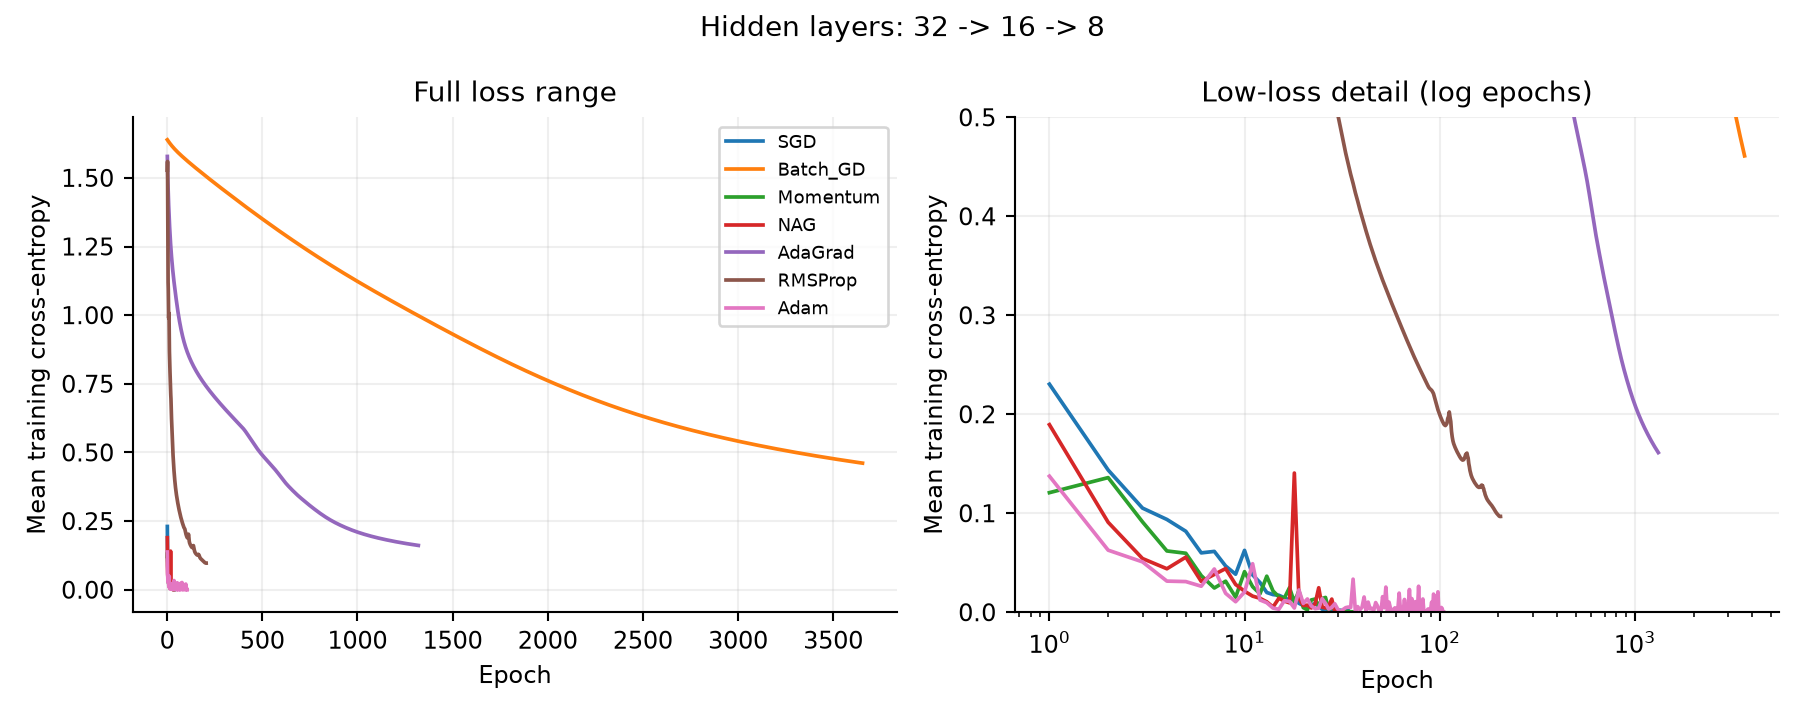
\includegraphics[width=\linewidth,height=0.36\textheight,keepaspectratio]{loss_3_layers.png}

\end{center}

{\small Superimposed post-epoch average training cross-entropy for all seven optimizers. The right panel magnifies losses below 0.5 with a logarithmic epoch axis; high-loss curves remain visible in the left panel.}\par

For this architecture, NAG has the highest validation accuracy, 97.89\%. The full curve, convergence loss difference, number of updates, and measured runtime are available in metrics.json.


\clearpage

\section{Results: 32 - 24 - 16 - 8}

\begingroup\small\setlength{\tabcolsep}{5pt}

\begin{tabularx}{\linewidth}{Yrrrrr}

\toprule

\textbf{Optimizer} & \textbf{Epochs} & \textbf{Train acc.} & \textbf{Val. acc.} & \textbf{Final CE} & \textbf{Final loss delta} \\

\midrule

SGD & 17 & 99.81\% & 96.89\% & 0.009842 & 9.38e-05 \\

Batch\_GD & 3957 & 86.42\% & 85.93\% & 0.453977 & 1.00e-04 \\

Momentum & 36 & 100.00\% & 97.81\% & 0.000085 & 2.29e-05 \\

NAG & 30 & 99.99\% & 97.89\% & 0.000288 & 7.03e-05 \\

AdaGrad & 1397 & 94.86\% & 93.62\% & 0.200351 & 9.97e-05 \\

RMSProp & 146 & 97.12\% & 95.73\% & 0.099436 & 4.15e-05 \\

Adam & 118 & 99.82\% & 97.52\% & 0.009932 & 6.13e-05 \\

\bottomrule\end{tabularx}\endgroup\par\medskip

\begin{center}

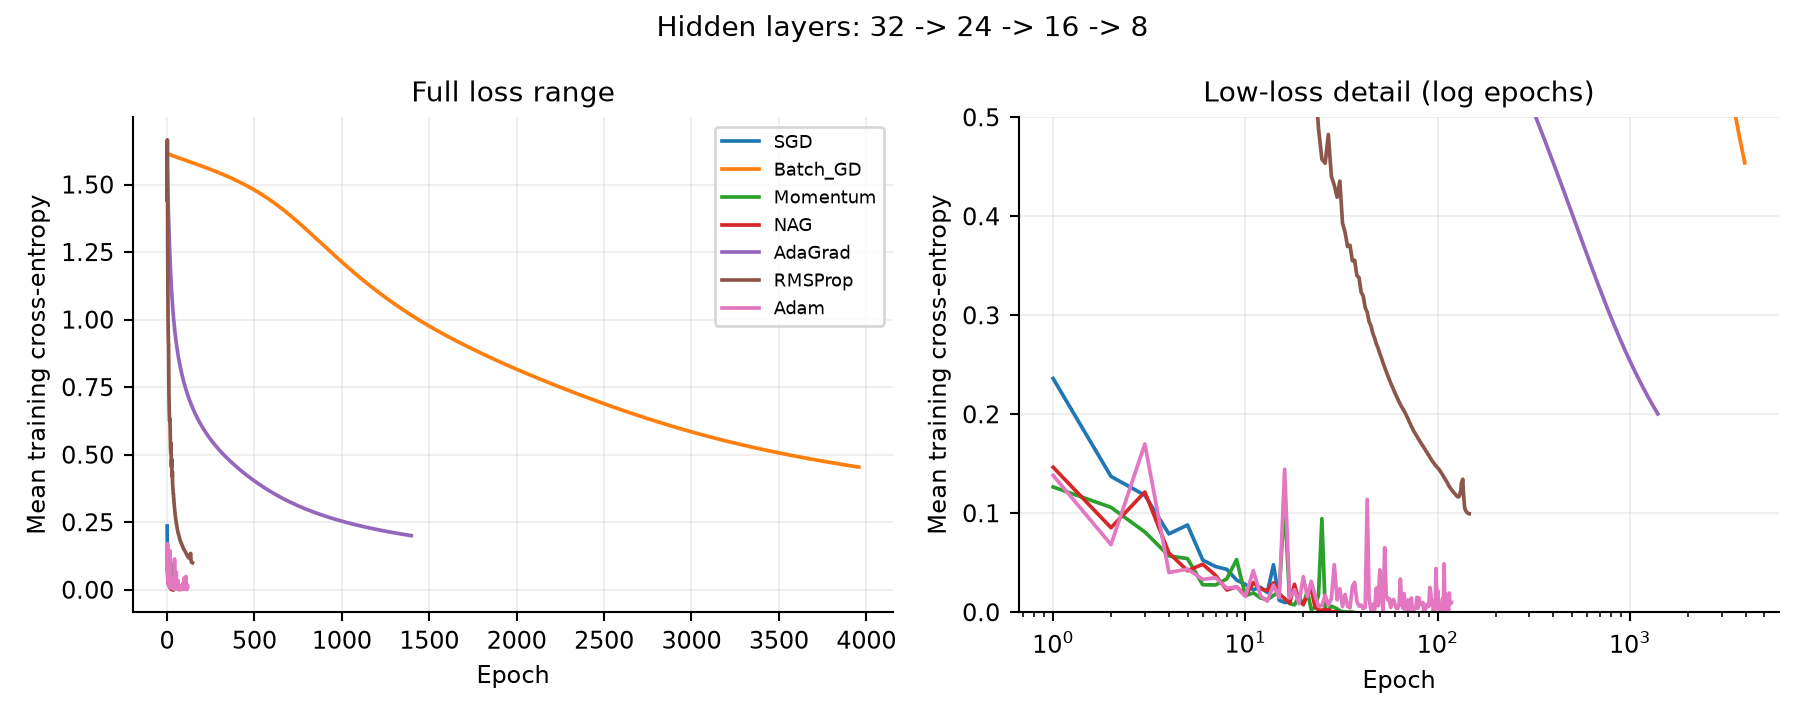
\includegraphics[width=\linewidth,height=0.36\textheight,keepaspectratio]{loss_4_layers.png}

\end{center}

{\small Superimposed post-epoch average training cross-entropy for all seven optimizers. The right panel magnifies losses below 0.5 with a logarithmic epoch axis; high-loss curves remain visible in the left panel.}\par

For this architecture, NAG has the highest validation accuracy, 97.89\%. The full curve, convergence loss difference, number of updates, and measured runtime are available in metrics.json.


\clearpage

\section{Results: 32 - 24 - 16 - 12 - 8}

\begingroup\small\setlength{\tabcolsep}{5pt}

\begin{tabularx}{\linewidth}{Yrrrrr}

\toprule

\textbf{Optimizer} & \textbf{Epochs} & \textbf{Train acc.} & \textbf{Val. acc.} & \textbf{Final CE} & \textbf{Final loss delta} \\

\midrule

SGD & 20 & 99.93\% & 97.31\% & 0.003807 & 9.63e-05 \\

Batch\_GD & 3448 & 89.75\% & 89.04\% & 0.346000 & 9.99e-05 \\

Momentum & 42 & 99.99\% & 97.55\% & 0.000303 & 3.27e-05 \\

NAG & 56 & 99.96\% & 97.52\% & 0.000860 & 6.70e-05 \\

AdaGrad & 1091 & 96.19\% & 94.73\% & 0.143059 & 9.99e-05 \\

RMSProp & 202 & 98.65\% & 96.31\% & 0.056387 & 3.71e-06 \\

Adam & 15 & 99.52\% & 97.52\% & 0.016955 & 5.36e-05 \\

\bottomrule\end{tabularx}\endgroup\par\medskip

\begin{center}

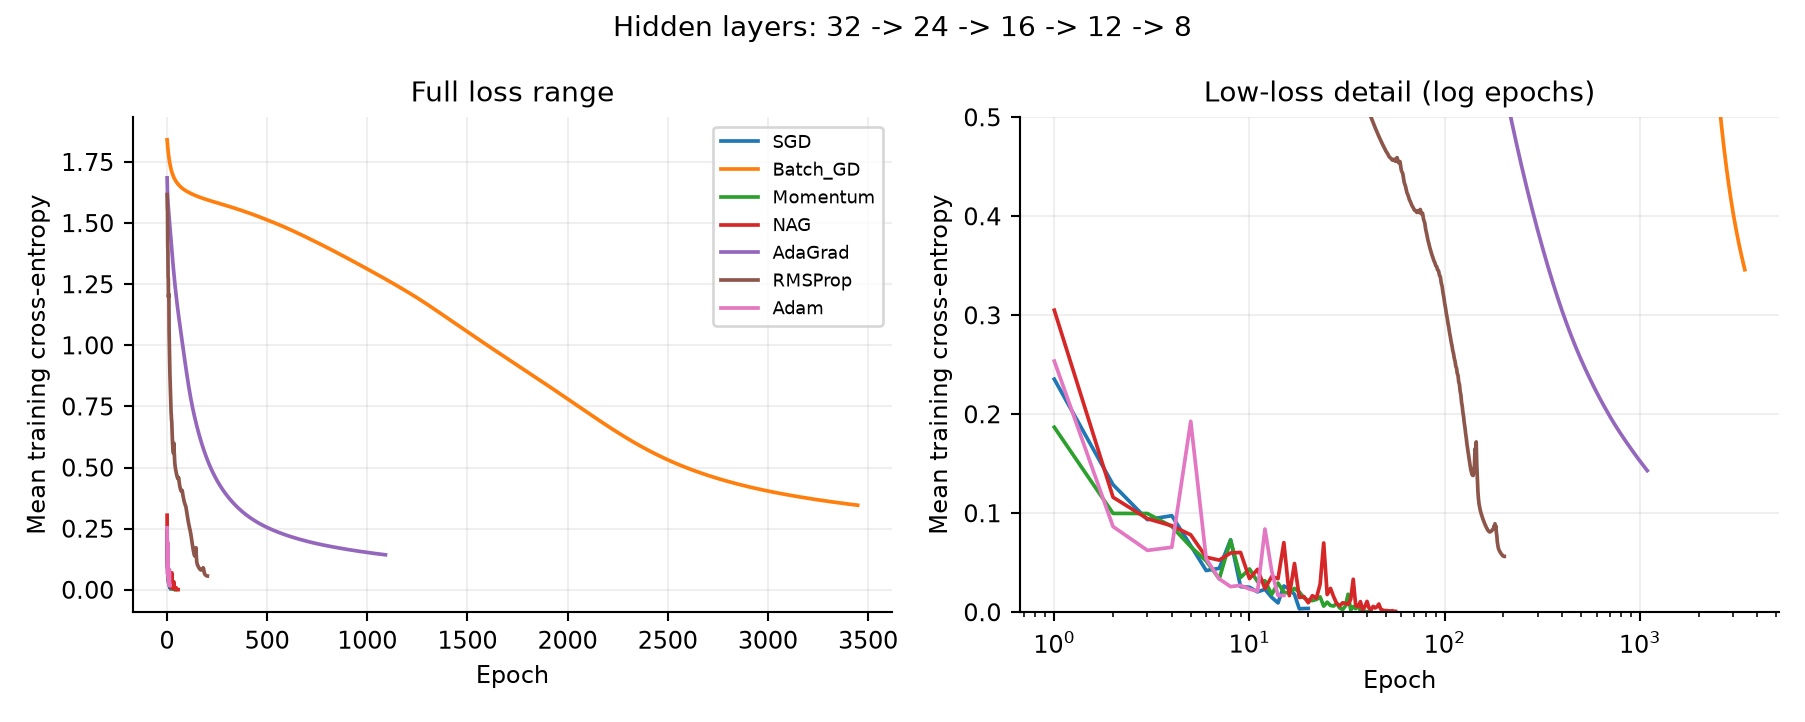
\includegraphics[width=\linewidth,height=0.36\textheight,keepaspectratio]{loss_5_layers.png}

\end{center}

{\small Superimposed post-epoch average training cross-entropy for all seven optimizers. The right panel magnifies losses below 0.5 with a logarithmic epoch axis; high-loss curves remain visible in the left panel.}\par

For this architecture, Momentum has the highest validation accuracy, 97.55\%. The full curve, convergence loss difference, number of updates, and measured runtime are available in metrics.json.


\clearpage

\section{Validation-selected model and test evaluation}

\begingroup\small\setlength{\tabcolsep}{5pt}

\begin{tabularx}{\linewidth}{lY}

\toprule

\textbf{Attribute} & \textbf{Selected result} \\

\midrule

Hidden layers & 32 $\to$ 16 $\to$ 8 \\

Optimizer & NAG \\

Convergence epochs & 32 \\

Training accuracy & 99.99\% \\

Validation accuracy & 97.89\% \\

Test accuracy & 97.87\% \\

\bottomrule\end{tabularx}\endgroup\par\medskip

\begin{center}

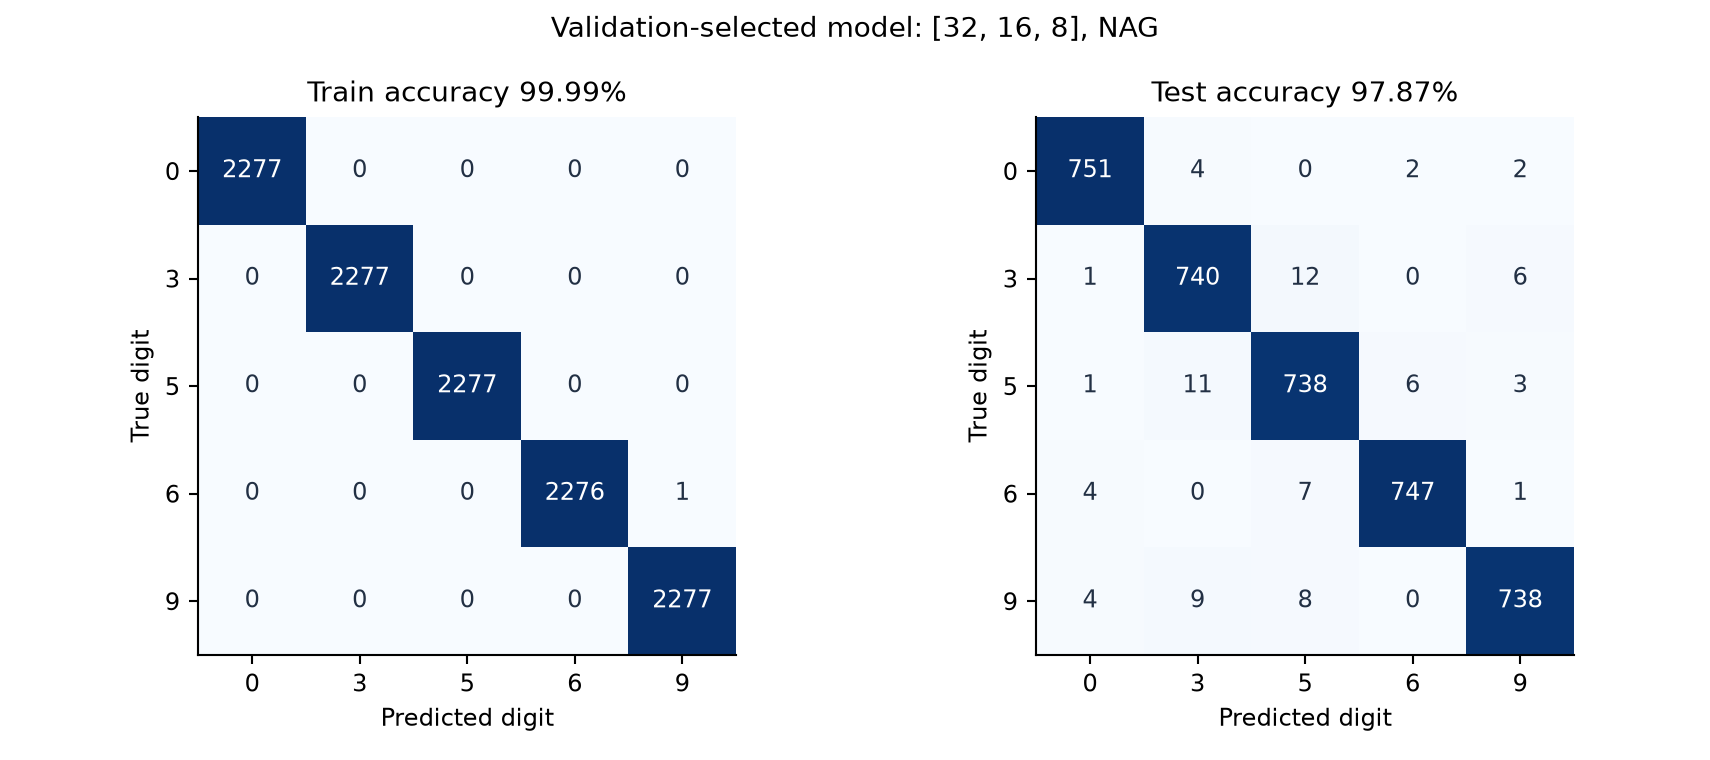
\includegraphics[width=\linewidth,height=0.43\textheight,keepaspectratio]{confusion_selected.png}

\end{center}

{\small Rows are true digits and columns are predicted digits. The training matrix has 2,277 observations per row; the test matrix has 759 per row.}\par

The largest directional test confusion is digit 3 predicted as 5 (12 images). The test split is used only after the final architecture and optimizer have been selected on validation accuracy; validation cross-entropy breaks an accuracy tie.


\clearpage

\section{Observations and reproducibility}

The comparison combines different update schedules because the brief explicitly prescribes them. Any performance gap therefore reflects both the optimizer and its assigned batch size. Identical initialization controls the starting point, but does not remove those scheduling differences. Small epoch-to-epoch loss changes also do not prove a minimum or high classification accuracy.


There is one seeded run per architecture and optimizer, not repeated trials. The tested compact widths are a finite architecture search, so the selected result is the best among these experiments. It is a fresh reproduction of Assignment 3, not a claim about a previously submitted model.


Source: \nolinkurl{CS601T_Assignment3_Details_07Sept2026.pdf}. The handout's printed date contains a year inconsistency; it does not change the experiment requirements.


Code folder: \texttt{Group32\_Assignment3\_code}.


Run \texttt{python run\_assignment3.py}, then \texttt{python verify\_results.py}. The measured comparison record is \nolinkurl{results/assignment3_best.json}.


Dataset SHA-256: \texttt{d973de54462a8f8710f74cb65d7b5670}\\ \texttt{993802b9252e531d78aaee19d93cb2a8}.


\end{document}
